\documentclass[]{article}
\usepackage[T1]{fontenc}
\usepackage{lmodern}
\usepackage{amssymb,amsmath}
\usepackage{ifxetex,ifluatex}
\usepackage{fixltx2e} % provides \textsubscript
% use upquote if available, for straight quotes in verbatim environments
\IfFileExists{upquote.sty}{\usepackage{upquote}}{}
\ifnum 0\ifxetex 1\fi\ifluatex 1\fi=0 % if pdftex
  \usepackage[utf8]{inputenc}
\else % if luatex or xelatex
  \ifxetex
    \usepackage{mathspec}
    \usepackage{xltxtra,xunicode}
  \else
    \usepackage{fontspec}
  \fi
  \defaultfontfeatures{Mapping=tex-text,Scale=MatchLowercase}
  \newcommand{\euro}{€}
\fi
% use microtype if available
\IfFileExists{microtype.sty}{\usepackage{microtype}}{}
\usepackage{longtable,booktabs}
\usepackage{graphicx}
% Redefine \includegraphics so that, unless explicit options are
% given, the image width will not exceed the width of the page.
% Images get their normal width if they fit onto the page, but
% are scaled down if they would overflow the margins.
\makeatletter
\def\ScaleIfNeeded{%
  \ifdim\Gin@nat@width>\linewidth
    \linewidth
  \else
    \Gin@nat@width
  \fi
}
\makeatother
\let\Oldincludegraphics\includegraphics
{%
 \catcode`\@=11\relax%
 \gdef\includegraphics{\@ifnextchar[{\Oldincludegraphics}{\Oldincludegraphics[width=\ScaleIfNeeded]}}%
}%
\ifxetex
  \usepackage[setpagesize=false, % page size defined by xetex
              unicode=false, % unicode breaks when used with xetex
              xetex]{hyperref}
\else
  \usepackage[unicode=true]{hyperref}
\fi
\hypersetup{breaklinks=true,
            bookmarks=true,
            pdfauthor={},
            pdftitle={},
            colorlinks=true,
            citecolor=blue,
            urlcolor=blue,
            linkcolor=magenta,
            pdfborder={0 0 0}}
\urlstyle{same}  % don't use monospace font for urls
\setlength{\parindent}{0pt}
\setlength{\parskip}{6pt plus 2pt minus 1pt}
\setlength{\emergencystretch}{3em}  % prevent overfull lines
\setcounter{secnumdepth}{0}
\usepackage{fancyhdr}
\pagestyle{fancy}
\lhead{C-Lyrics - A Word Cloud for Lyrics}
\rhead{\thepage}
\cfoot{Team 6}
\renewcommand{\headrulewidth}{0.4pt}
\renewcommand{\footrulewidth}{0.4pt}

\title{PaperCloud}
\author{Justine Cocchi\\jcocchi@usc.edu \and Kelsey Fargas\\kfargas@usc.edu \and Mark Krant \\ mkrant@usc.edu\and Milad Gueramian\\gueramia@usc.edu \and Jeff Kang\\kangjr@usc.edu \and Séb Arnold\\arnolds@usc.edu}
\date{6 April 2015}

\title{%
	PaperCloud \\
	\large First Iteration Report}

\begin{document}

\clearpage\maketitle
\thispagestyle{empty}

\pagebreak

\tableofcontents
\setcounter{tocdepth}{3}
\thispagestyle{empty}

\pagebreak

\section{Executive Summary}\label{executive-summary}

PaperCloud is an internet application on the world wide web, built for
the purpose of organizing words from different researchers' publications
into a word cloud. The publications come exclusively from IEEE and ACM.
This application will allow for the generation of 2 types of clouds and
as such, two types of searches for each cloud. The first is to enter the
full name of the researcher. PaperCloud will then generate a word cloud
(if the input is valid) based on all the MaxWord most common words from
the researcher's papers. The second search option allows the user to
enter a keyword phrase which will result in a wordcloud consisting of
the MaxWords most common words from all the documents searchable (from
the two publications mentioned) containing the keywords. PaperCloud
offers certain other features to simplify further searches and word
cloud generations which are described in the rest of this document.

\pagebreak

\section{1 Introduction}\label{introduction}

\subsection{1.1 Purpose}\label{purpose}

The purpose of this document is to clearly describe every aspect of the
second group project for the CSCI-310 course taken at the University of
Southern California in the Spring semester of the year 2015. The
intended audiences of this software requirements specification document
includes, but is not limited to: the members of group six whose names
are listed on the front page of this document and by whom this document
is prepared, the professor of the course Dr.~William G. Halfond, and the
teaching assistant Sonal Mahajan. Other possible audiences include:
students who are at the time of this publication taking the course in
which this project is assigned or any future students of this course who
may read this document should it become available to them by the course
instructor Dr.~William G. Halfond or by any other means which cannot be
predicted at this time. This software development project will hereafter
be referred to as PaperCloud. It is intended for any user with an
internet connection-either through a mobile or stationary platform.

\subsection{1.2 Overview}\label{overview}

This document is to present the management and development structure of
the first iteration of software under construction. The different
processes are explained in detail in the following sections.
Furthermore, the project serves as guide on how to build software using
the SCRUM and Extreme Programming practices of the Agile collection of
processes.

The content regards the two Agile collection development processes
described above. Section 2 elaborates on our use of SCRUM which includes
our project management plan and organization. Section 3 and 4 details
our requirements, design, and implementation planning. Section 5
describes the review process in which we reevaluate the effectiveness of
our strategy and implementation. The Appendix includes some artifacts
and further details on our development process as a whole.

\subsection{1.3 References}\label{references}

{[}1{]} Cunningham, Ward. ``Extreme Programming''. O'Reilly Media. July
2003.

{[}2{]} Wells, Don. ``Extreme Programming''. October 10,2013. April 5,
2015.\url{http://www.extremeprogramming.org/}.

\subsection{1.4 Terminology}\label{terminology}

IEEE- Institute of Electrical and Electronics Engineers ACM- Association
of Computing Machinery Development team (use same as before) SCRUM XP-
Extreme Programming Asana- Planning and time tracking software available
on the internet. arXiv- application provide by Cornell university that
helps with searching for research papers across a wide range of
subjects. Gmail- Email messaging software from Google Inc. Used for
communication purposes by development team Clients/Customers - Professor
William G. Halfond and Sonal Mahajan


\begin{longtable}[c]{@{}ll@{}}
\toprule\addlinespace
\begin{minipage}[t]{0.47\columnwidth}\raggedright
Term
\end{minipage} & \begin{minipage}[t]{0.47\columnwidth}\raggedright
Definition
\end{minipage}
\\
\hline
\\\addlinespace
\begin{minipage}[t]{0.47\columnwidth}\raggedright
IEEE
\end{minipage} & \begin{minipage}[t]{0.47\columnwidth}\raggedright
Institute of Electrical and Electronics Engineers
\end{minipage}
\\\addlinespace
\begin{minipage}[t]{0.47\columnwidth}\raggedright
ACM
\end{minipage} & \begin{minipage}[t]{0.47\columnwidth}\raggedright
Association of Computing Machinery
\end{minipage}
\\\addlinespace
\begin{minipage}[t]{0.47\columnwidth}\raggedright
Development team
\end{minipage} & \begin{minipage}[t]{0.47\columnwidth}\raggedright
All of the individuals whose names appear on the cover of this document.
These persons have collectively put this document together and will
collectively implement the software product described in subsequent
sections.
\end{minipage}
\\\addlinespace
\begin{minipage}[t]{0.47\columnwidth}\raggedright
XP
\end{minipage} & \begin{minipage}[t]{0.47\columnwidth}\raggedright
Extreme Programming
\end{minipage}
\\\addlinespace
\begin{minipage}[t]{0.47\columnwidth}\raggedright
Asana
\end{minipage} & \begin{minipage}[t]{0.47\columnwidth}\raggedright
Online planning and time tracking software
\end{minipage}
\\\addlinespace
\begin{minipage}[t]{0.47\columnwidth}\raggedright
arXiv
\end{minipage} & \begin{minipage}[t]{0.47\columnwidth}\raggedright
Application provided by Cornell university that helps with searching for research papers across a wide range of subjects.
\end{minipage}
\\\addlinespace
\begin{minipage}[t]{0.47\columnwidth}\raggedright
Gmail
\end{minipage} & \begin{minipage}[t]{0.47\columnwidth}\raggedright
Email messaging software from Google Inc. Used for communication purposes by development team
\end{minipage}
\\\addlinespace
\begin{minipage}[t]{0.47\columnwidth}\raggedright
Clients/Customers
\end{minipage} & \begin{minipage}[t]{0.47\columnwidth}\raggedright
Professor William G. Halfond and Sonal Mahajan
\end{minipage}
\\\addlinespace
\bottomrule
\end{longtable}


\subsection{1.5 Scope}\label{scope}

PaperCloud is a web based application for generating a horizontally
positioned text word cloud generated from the most commonly occurring
words from a collection of research papers. There are two search options
each correlating to two different clouds that can be generated. In the
first option, the cloud is generated based on the first and last name
search for a particular author. The second search option allows the user
to enter a keyword phrase which results in a word cloud generated based
on words from all articles that contain the keyword phrase.

PaperCloud will be hosted and available to the World Wide Web and will
require no user registration or membership. To access the PaperCloud
service, a user only needs an internet connection and one of the
commonly used web browsers. PaperCloud arXiv API to generate the results
from

\subsection{1.6 Documents}\label{documents}

We used certain third party software products to assists with project
management and implementation. Information for access to these products
can be found below. Asana is used to keep project backlogs and iteration
related scheduling and task completion details for each sprint. Each
member of the development team will chose tasks from the sprint log to
complete and can interact with other member and update information about
task progress on Asana.

For full access to SCRUM meeting notes refer to the Group 6 discussion
board on the course BlackBoard link under the ``Iteration 1 Team
Activity Log'' thread. For a quick reference, refer to the appendix
Section 6.1.

For full access to Asana, the clients are suggested to refer to their
University of Southern California Gmail account where they will find an
invitation to view PaperCloud's Asana account.

For full access to source code, please refer to the project's public
Github page at:

\begin{itemize}
\itemsep1pt\parskip0pt\parsep0pt
\item
  https://github.com/C-Lyrics/PaperCloud
\end{itemize}

\section{2 SCRUM Management}\label{scrum-management}

\subsection{2.1 Process Introduction}\label{process-introduction}

The primary purpose of using Scrum is to work together to develop the
product required from the client. In doing so, we broke up the
requirements created in the back log. This way, we were able to
prioritize tasks for the sprint log to better understand which tasks
needed to be completed before others. By building the product in smaller
broken down pieces, the development team was able to give feedback and
changes if necessary.

The Scrum process is comprised of three different procedures: pre-game,
mid-game, and post-game. The pre-game process involves engaging in
planning and high-level design. This included elicitation of the
requirements from the client, and the Scrum spring cycle. This comprised
of the delegation of the three main roles, such as Scrum master, Product
owner, and team, and organizing meeting times with the development team.
After clarifying the requirements, the development team created the
product backlog and sprint log. Every member present at each meeting
that occurred answered the workday questions to make sure the everyone
was on track for task completion. The mid-game process involves
developing, wrapping, reviewing, and adjusting. This is primarily
abiding by the sprint logs that were created from the backlogs. We
developed and wrapped code, reviewed code by pair programming, and make
adjustments accordingly. The post-game process involved closure of the
first iteration, which includes the sprint review and sprint
retrospective.

\subsection{2.2 Organisation Planning}\label{organisation-planning}

\subsubsection{2.2.1 Roles}\label{roles}

The group divided the roles in the following manner:

\begin{itemize}
\itemsep1pt\parskip0pt\parsep0pt
\item
  SCRUM Master: Justine
\item
  Product Owners: Sonal Mahajan
\item
  Customers: Sonal Mahajan, William Halfond
\item
  Development Team: Sebastien, Mark, Milad, Justine, Jeff, Kelsey
\end{itemize}

Justine was chosen by consensus to be our SCRUM master because she would
be available to attend all meetings and she has had experience using
SCRUM techniques.

\subsubsection{2.2.2 Teams}\label{teams}

The teams are allocated as the following:

\begin{itemize}
\itemsep1pt\parskip0pt\parsep0pt
\item
  Frontend: Sebastien, Kelsey, Justine
\item
  Backend: Mark, Milad, Jeff
\end{itemize}

These teams were chosen based on the team allocations we used in the
previous project, as well as each group member's individual coding
knowledge and experience. We felt that the division of frontend and
backend made sense as we could assign requirements for implementation on
the frontend Javascript and HTML code and the backend PHP code.

\subsubsection{2.2.3 Product Backlog and Sprint
Logs}\label{product-backlog-and-sprint-logs}

Asana was used to create a product backlog of project requirements that
were determined based on meetings with the customer. From this product
backlog, we narrowed the list down to a sprint log for our first
iteration of code. The sprint log was further broken down into
implementable tasks that were outlined on Asana, which allowed us to
track the development progress of our first sprint.

\begin{itemize}
\item
  Product Backlog

  \begin{itemize}
  \itemsep1pt\parskip0pt\parsep0pt
  \item
    Search by keyword
  \item
    Search by researcher
  \item
    Autocomplete for searching by researcher
  \item
    Ability to see history of searches
  \item
    Display word cloud with common words from top N pages
  \item
    Progress bar for progress of generating word cloud
  \item
    Click on word in cloud lets you make new search with that word
  \item
    Click on word in cloud lets you see all research papers with that
    word in it and how frequently the word appears in each one
  \item
    Display list of research papers that contain selected word in them
    with their authors listed next to them in MLA format
  \item
    Click research paper title takes you to a page with a link to
    download the paper
  \item
    Click author name in research paper list takes you to word cloud
    generation of common words from that author's research papers
  \item
    Select research papers to export references in .txt and .pdf format
  \item
    Ability to get BIBTEX reference of each research paper upon hover/
    button press
  \item
    Navigation buttons between all pages
  \end{itemize}
\item
  Sprint Backlog: Because the product owner was not present at our
  sprint planning meeting due to meeting logistics, we were not able to
  produce a sprint backlog during this meeting. However, we requested a
  prioritized list of requirements and were able to create the sprint
  backlog laid out below at our first scrum meeting on March 27th.

  \begin{itemize}
  \itemsep1pt\parskip0pt\parsep0pt
  \item
    Search by researcher: implement researcher search function, make API
    call with researcher name
  \item
    Search by keyword: implement keyword search function, make API call
    with keyword, parse PDF's with PHP, get abstract from API
  \item
    Display word cloud with common words from top N pages: implement
    function to gather common words from top N pages, display word cloud
  \item
    Progress bar for progress of generating word cloud
  \item
    Click on word in cloud lets you make new search with that word: make
    wordcloud results clickable, run search function with new keyword,
    make API call with new keyword
  \end{itemize}
\end{itemize}

\begin{figure}[htbp]
\centering
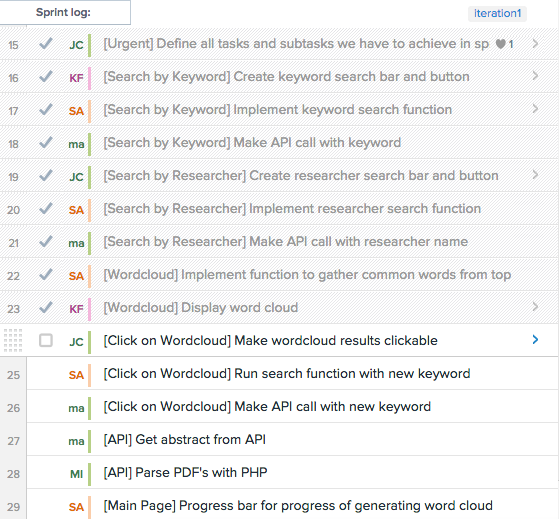
\includegraphics{sprintlogv2.png}
\caption{The Sprintlog for Iteration 1, including the task attribution}
\end{figure}

\subsection{2.3 Meetings}\label{meetings}
\begin{figure}[htbp]
\centering
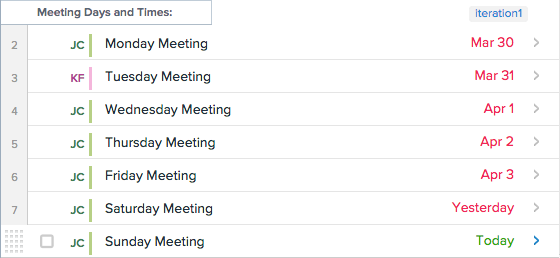
\includegraphics{meetings.png}
\caption{Meeting Times}
\end{figure}

Our team had a sprint planning meeting on Thursday March 26th in which
we set up various future group meeting times for the week of our
implementation phase. These meeting times are documented in Asana. All
team members then signed up to participate in four to five meetings
based on their availabilities. In this process, we were able to have
rotating teams to allow for variance in our pair programming practices
while keeping in line with having the team meet every day.

\begin{figure}[htbp]
\centering
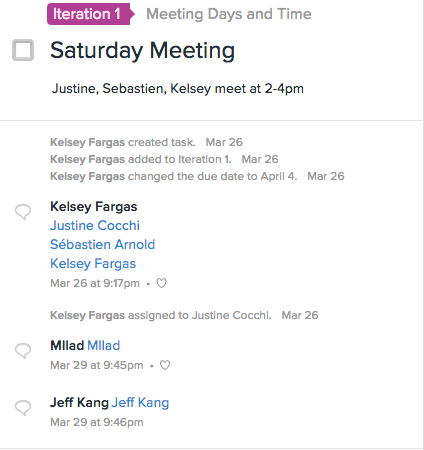
\includegraphics{SatMeeting.png}
\caption{Example of Scheduled Meeting}
\end{figure}

\section{3 Extreme Programming
Practices}\label{extreme-programming-practices}

Extreme programming (XP) is an agile software engineering methodology
which enforces several practices. It is a natural companion to the SCRUM
process, as both of them are iterative and organized in sprints and
iterations.

In addition to extending Agile practices to the extreme, XP also
promotes its own values and assumptions. The values include:

\begin{itemize}
\itemsep1pt\parskip0pt\parsep0pt
\item
  \textbf{Communication}: Communication is essential for adjusting to
  feedback and implementing constant changes. Honest, regular
  communication should not only happen amongst developers, but also
  amongst their customers.
\item
  \textbf{Feedback}: Feedback is the response from the customer to
  clarify what is required and wanted. By asking questions and making
  adjustments accordingly, the development team will be able to ensure
  that the code complies with the customer's specifications.
\item
  \textbf{Simplicity}: The development team should only focus on what
  really needs to be built and only solve the current problems of the
  day.
\item
  \textbf{Courage}: In this case, courage means making difficult
  decisions when necessary. It could be easy to disregard an issue
  because it would make several people unhappy. Courage implies speaking
  up and pointing out difficulties.
\end{itemize}

Extreme programming not only assumes that each stakeholder will
incorporate the mentioned values, but also makes the following
assumptions:

\begin{itemize}
\itemsep1pt\parskip0pt\parsep0pt
\item
  \textbf{Enough Time and Resources}: Instead of rushing through the
  coding process, XP enables developers to work at their normal paces.
  By working in very short cycles, it reduces the length of time between
  actions and their effects. It also adjusts the project to fit the
  available resources.
\item
  \textbf{Constant Cost of Change}: XP ensures a constant change of
  cost. This means that implementing a functionality now versus in a
  year will take the same amount of effort. By making this assumption,
  it allows developers to focus on current tasks without worrying about
  future features.
\item
  \textbf{Developper Effectiveness}: Extreme programming assumes that in
  order to have great software, the developers should be great as well.
\item
  \textbf{Freedom to Experiment}: Every team member (including managers,
  developers, and customers) should have the opportunity to experiment.
  This means asking question such as ``Is there a better way to solve
  this problem ?'' and keeping an open mind towards the answers.
\end{itemize}

\subsection{3.1 Coding Practices}\label{coding-practices}

\subsubsection{3.1.1 Simple Code and
Design}\label{simple-code-and-design}

Simple code and design was practiced to make code more efficient and
straightforward. The development started by defining what frameworks to
use and choosing the ones that are most flexible with respect to change
of direction for long term purposes. These frameworks were chosen to be
AngularJS and Slim. The development team also implemented features using
libraries and reused code, taking out unnecessary functionalities when
needed. This is shown in the comparison of code from C-Lyrics - a team's
previous project - and PaperCloud, as well as the use of jqcloud2.
However, the two pages for listing display were created, although they
are not XP-friendly.

\subsubsection{3.1.2 Refactor Mercilessly}\label{refactor-mercilessly}

The purpose of refactoring is to have better and more efficient code.
This is a crucial step in order to obtain readable code and reduce the
cost of change. The developing team's last programming session was
entirely devoted to refactoring. The goal was to improve code's
readability, document some of the main functions, and remove superficial
or unused functionalities. Refactoring can be seen in the last commits
on the git repository.

\begin{figure}[htbp]
\centering
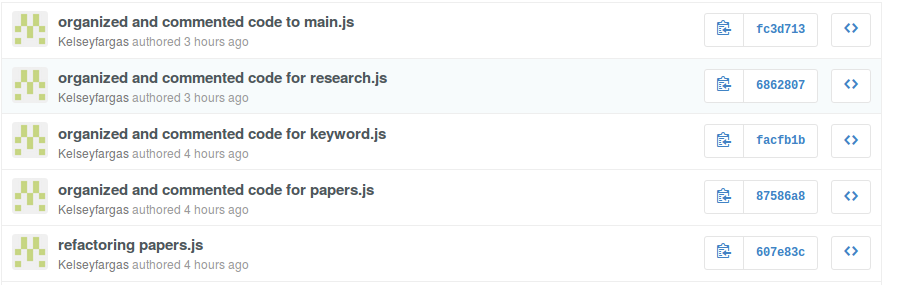
\includegraphics{refactor_commits.png}
\caption{Refactor Commits}
\end{figure}

\subsubsection{3.1.3 Coding Standards}\label{coding-standards}

Coding standards are required to enable readability and communication
through code. By having everyone writing code in the same manner, the
team ensures that any developer will have some degree of familiarity
with the whole codebase. The developers used custom code formatting
templates to ensure homogeneity over the entire code. The code is openly
available on GitHub as mentioned in Section 1.6, and the formatting
templates are available at:

\begin{itemize}
\itemsep1pt\parskip0pt\parsep0pt
\item
  https://github.com/seba-1511/st\_settings
\end{itemize}

\subsubsection{3.1.4 Common Metaphor}\label{common-metaphor}

The idea behind having a common metaphor is to describe the project as
it evolves. It allows the development team to share a vocabulary that
will define well-understood relationships. For this project, the
development team used a previous project as a metaphor. While not being
the most creative, this was highly useful as every team member was able
to clearly visualize the different parts of the application and how they
related to each other. The specific project was the creation of a lyrics
retrieval website which offered a lot of similar functionalities to the
current project.

\subsection{3.2 Developer Practices}\label{developer-practices}

\subsubsection{3.2.1 Test Driven
Development}\label{test-driven-development}

\begin{figure}[htbp]
\centering
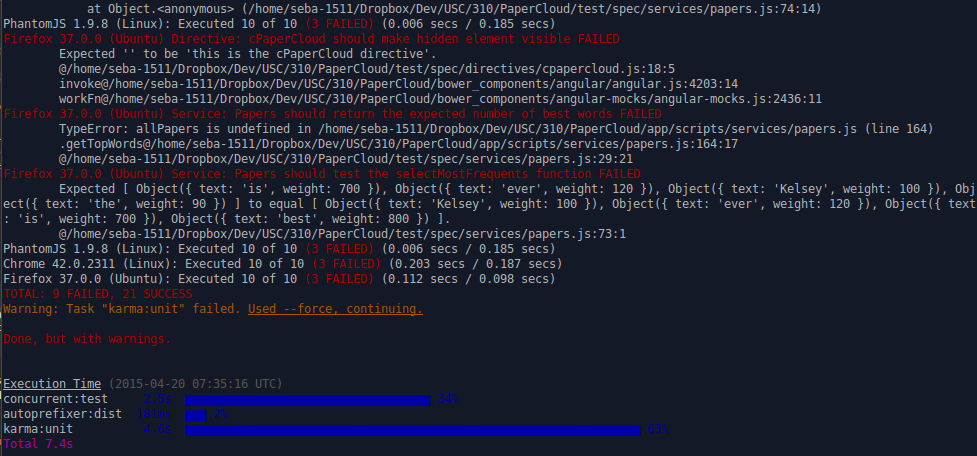
\includegraphics{test_output.png}
\caption{Example of test output}
\end{figure}

Before implementing any functionality, we first wrote unit tests for
functional requirements or end-to-end tests for visual requirements.
This practice is underlined in our GitHub commit history. Due to the absence of a customer in our team,
we do not consider these tests as acceptance tests. However, the visual
tests were developed using the same framework and methodology that the
customer would be using for acceptance testing.

\begin{figure}[htbp]
\centering
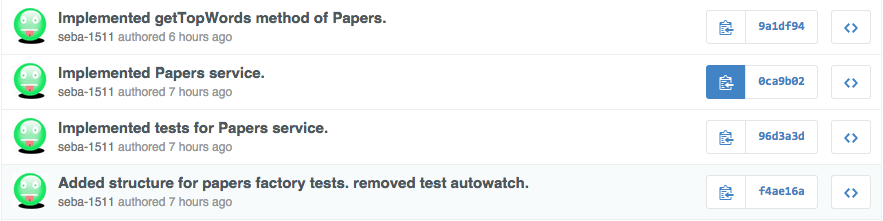
\includegraphics{tdd_proof.png}
\caption{Typical Test Driven Development}
\end{figure}

\subsubsection{3.2.2 Pair Programming}\label{pair-programming}

\begin{figure}[htbp]
\centering
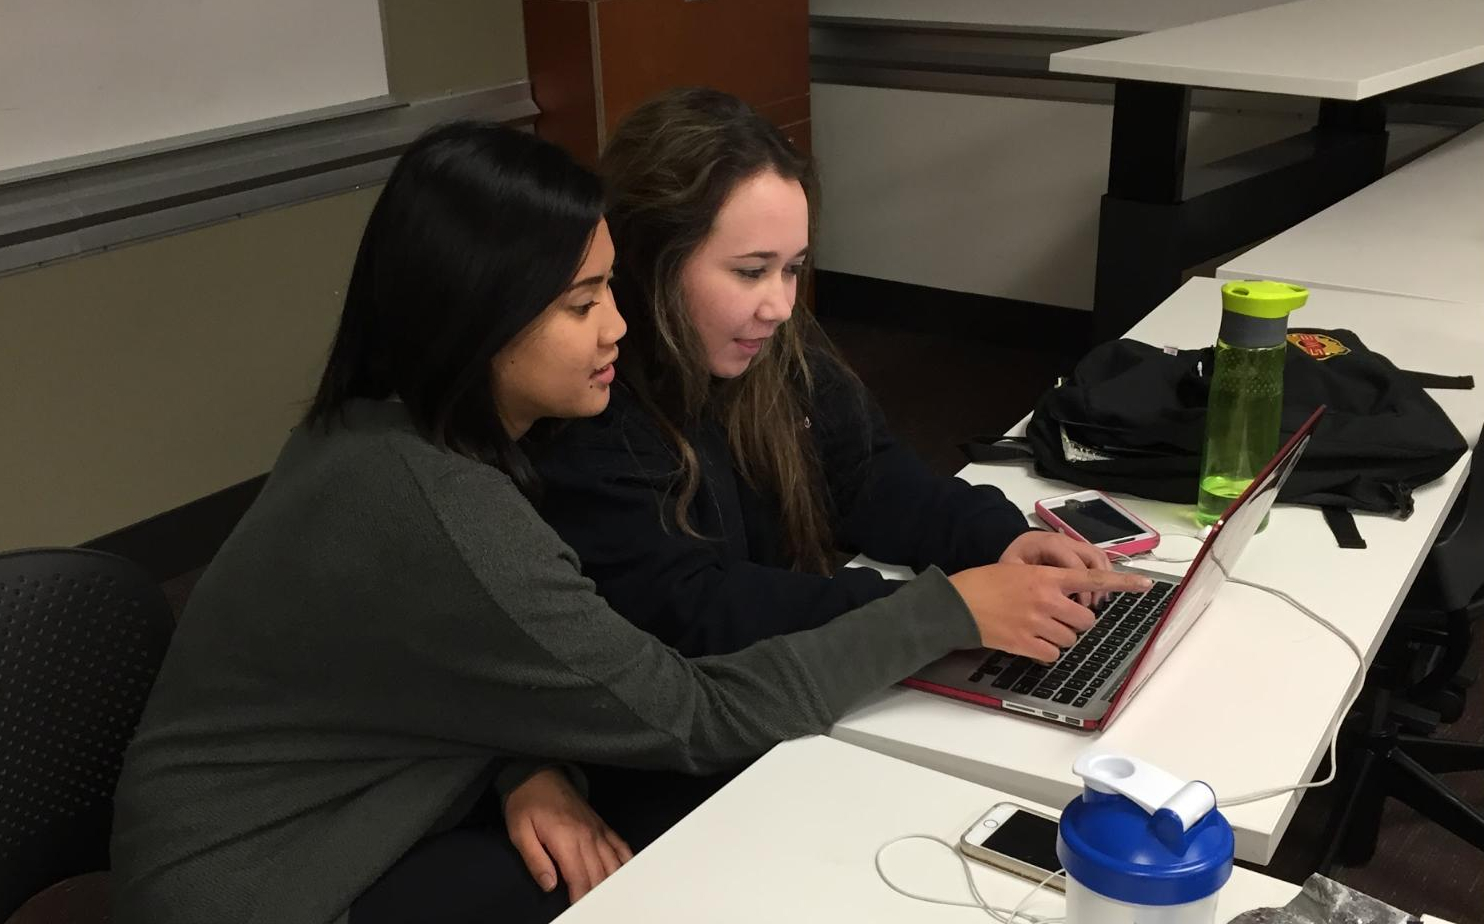
\includegraphics{serious_pair_prog.jpg}
\caption{Team Members Pair Programming}
\end{figure}

Pair programming is the process of programming in pairs with separate
roles: driver and observer. The driver writes code actively, while the
observer passively guides and discusses the code being written with the
driver. During all of our team meetings, we made sure that at least two
team members were engaging in pair programming. This practice provides
two significant benefits: uniformization of code throughout the project
and collective code ownership. The team reported who pair programmed on the forum thread, and took pictures of team members in a pair programming session.

\subsubsection{3.2.3 Collective Code
Ownership}\label{collective-code-ownership}

Collective code ownership was created within respective teams, for
example Kelsey, Sebastien, and Justine worked on the same GitHub
repository as a part of the frontend team. Ultimately, there was little
communication between the frontend and backend teams of our group. The
team essentially only defined what the API should look like and worked
on separate code repositories.

\subsubsection{3.2.4 Continuous
Integration}\label{continuous-integration}

To apply continuous integration, our team set up a GitHub account and
TravisCI. This allowed us to consistently make sure that we all shared
the same code base, and it allowed us to monitor which commits broke our
tests. This is underlined by the team's constant use of GitHub.


\begin{figure}[htbp]
\centering
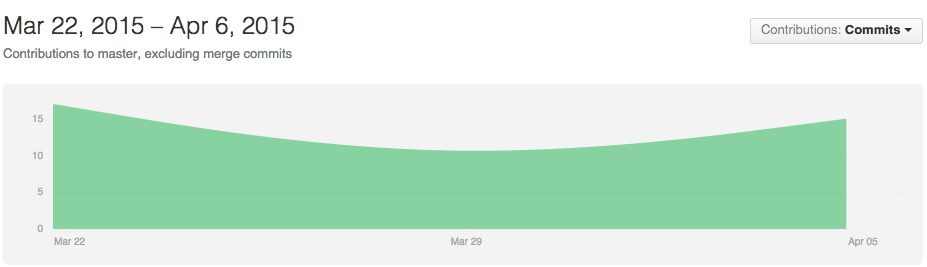
\includegraphics{steady_pace.png}
\caption{Constant Use of GitHub}
\end{figure}

\subsection{3.3 Business Practices}\label{business-practices}

\subsubsection{3.3.1 Customer Team Member}\label{customer-team-member}

One of the main obstacles of adhering to Extreme programming practices
was the fact that it was not possible to have the customer as a team
member due to the special circumstances of the project being completed
in a class environment. Instead of working closely with the customer
during our meetings, the team focused on separate meetings with the
customer and inferred preferences from conversations through Blackboard
and in-person meetings.


\begin{figure}[htbp]
\centering
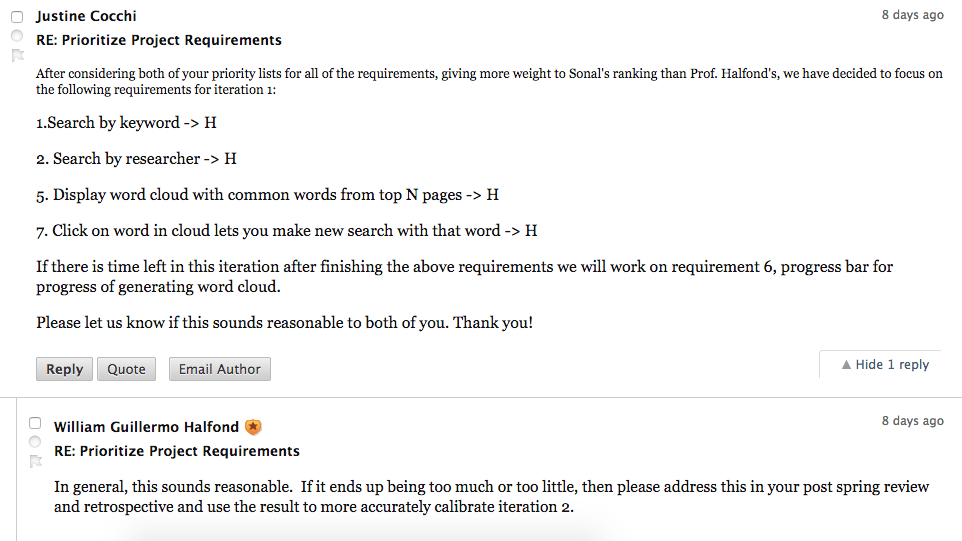
\includegraphics{sm_conv.png}
\caption{Conversation Between the SCRUM Master and a Customer}
\end{figure}

\subsubsection{3.3.2 Planning Game and User
Stories}\label{planning-game-and-user-stories}

The planning game was played through the scrum master, Justine. She made
an early decision on which functionalities would be implemented for this
iteration, according to the customer's defined product backlog. We
stated a set of sprint logs that was a filtered version of the product
backlog to complete high priority tasks first. These sprint logs also
served to break down backlog requirements into implementable processes.

\subsubsection{3.3.3 Regular Releases}\label{regular-releases}

After this first iteration, the team can now submit a fully working and
tested system. This will hopefully be the case for next iterations,
which will allow for regular releases. As outlined in the iteration
review, we overestimated our capacities with respect to our sprint log.
However, after the final refactoring, the requirements we decided to
tackle are fully completed, and modifying the implemented functions will
only occur if new functionalities are to be added that conflict with
pre-existing functionalities.

\subsubsection{3.3.4 Sustainable Pace}\label{sustainable-pace}

The team held meetings every day in the past week, for an average time
of 2 hours. We did not necessarily have to ``rush'' or overwork
ourselves. This is underlined by GitHub's graph, which shows a steady
pace which can be shown in the figure below. Interestingly, however, as several team members were progressing on different tasks, most of tasks were marked
as complete at the same time. This is shown in the figure by the
Burndown chart in Asana. Please note that the following Burndown includes tasks such as meetings, best practices and other non-sprint related tasks, which were not checked off. The final count of remaining tasks is 13, while 9 were effectively completed.

\begin{figure}[htbp]
\centering
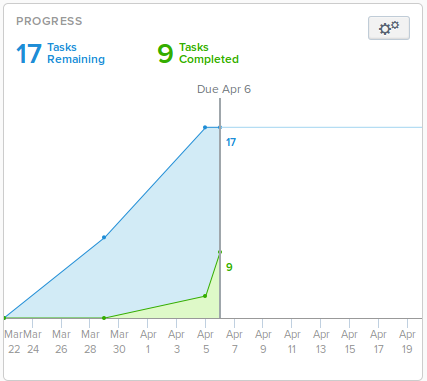
\includegraphics{burndown.png}
\caption{Burndown Chart}
\end{figure}

\subsection{4 Artifacts}\label{artifacts}

\subsubsection{4.1 Story Cards}\label{story-cards}

Although the customer was not necessarily available for the writing of
story cards, the following cards have been created from the project
requirements addressed in this iteration. If story cards were used as a
strategy for requirements engineering, the customer would have arranged
these in order of importance for prioritization.

Users should be able to search by keyword for articles Users should be
able to search by researcher name for articles A wordcloud should appear
after a search has been completed Clicking on a word in the wordcloud
should perform a new search with that keyword A progress bar should show
what progress of the word cloud being generated

\subsubsection{4.2 The Bullpen}\label{the-bullpen}

In order to simulate an effective bullpen, our team booked rooms in
Leavey library for our meetings. In accordance with bullpen strategies,
these rooms are isolated, and team members have laptop computers to move
around freely and engage in pair programming. We were not, however, able
to have the customer in the room with us to ask clarifying questions.

\section{5 Iteration Review}\label{iteration-review}

\subsection{5.1 Sprint Review}\label{sprint-review}

Our sprint review took place at a development team meeting on April 5th
with all members present. We discussed the completed items on our
product and sprint backlogs as well as the timeline for future progress
with this project.

While the sprint review traditionally has the product owner present,
this was not plausible for us because our meeting occurred after all
changes to the code were made on Sunday night when the product owner was
not available. To compensate for this, we extensively met with the product owner on Monday April 6th, and had an additional retrospective meeting on Tuesday April 7th.

\subsubsection{5.1.1 Completed Product Backlog
Items}\label{completed-product-backlog-items}

Below is a list of completed product backlog items: 

* Search by keyword \\
* Search by researcher \\

\subsubsection{5.1.2 Completed Sprint Backlog
Items}\label{completed-sprint-backlog-items}

Below is a list of completed sprint backlog items: * Search by keyword:
implement researcher search function, make API call with researcher name
* Search by keyword: implement keyword search function, make API call
with keyword, parse PDF's with PHP, get the abstract from API

\subsubsection{5.1.3 Timeline}\label{timeline}

Based on the current state of the product backlog, the development team
is behind schedule. They will need to improve the efficiency of meetings
by adhering to more XP principals and by sticking closely to all of the
scrum and agile development guidelines. Next sprint, the development
team plans to catch up on the product and sprint backlogs, as well as
continue adding functionality to the system.

\subsection{5.2 Sprint Retrospective}\label{sprint-retrospective}

The development team's sprint retrospective took place at a development
team meeting on April 5th at 6:00pm with all members present.

\subsubsection{5.2.1 Identify What Went
Well}\label{identify-what-went-well}

The development team was successfully able to have at least three
members meet every day. This allowed the development team to make steady
progress towards completion of this sprint's goal. The team worked well
together and were able to split up jobs based on each team member's
strengths to optimize time.

\subsubsection{5.2.2 Identify What Needs
Improvement}\label{identify-what-needs-improvement}

In the next sprint the development team need to break down the sprint
log into much smaller, more manageable tasks. Because there were large
tasks in the backlog, different people worked on each one, finishing the
majority of tasks at the same time instead of finishing a steady stream
of log items within the sprint. This will change the structure of the
sprint meeting minutes because we will be able to be more specific in
our goals for the day instead of making general statements about what we
have worked on and what we plan to work on that day. Doing so will help
the team adhere to agile development much more closely and will
hopefully increase efficiency and help to keep all of the team members
better informed on each other's work. The team will also be able to see
project progress much more clearly and will know how to adjust the
sprint backlog for the next iteration to match the work pace to
productivity.

\subsubsection{5.2.3 Plan to Improve Process Next
Sprint}\label{plan-to-improve-process-next-sprint}

For the next sprint the development team plans to meet with the product
owner earlier in the process and get a better idea of what is reasonable
to add to the sprint backlog. They will also attempt to have scrum
meetings with the whole team as opposed to only having meetings with the
three plus people that worked on the project that day. In doing so the
development team will be better equipped to adjust the sprint backlog
throughout the iteration to ensure that the team is neither overwhelmed
or not working to its full potential.

\subsection{5.3 Scrum Meetings Review}\label{scrum-meetings-review}

All scrum meeting minutes can be found with timestamps on the online
blackboard forum for team 6 in the ``Iteration 1 Team Activity Log''
thread. Additionally, all of the meeting minutes are listed in the
Appendix in section 6.1 for the stakeholders' convenience.

\subsection{5.4 Customer Integration
Review}\label{customer-integration-review}

The development team met with the customers, Professor William G.
Halfond and Sonal Mahajan, to obtain the necessary requirements for the
intended project. After getting the initial set of requirements from
both of the customers, the development team used this information to
build the product backlog. The development team then asked for the
customers to prioritize all of the requirements so they could build the
sprint backlog for this iteration. The sprint backlog was checked with
the customers to ensure that they agree that the decided tasks are
reasonable for this sprint.

Later in the sprint the development team met again with Sonal, the
product owner, to confirm that none of the product requirements had
changed. While there were changes to be made to the product backlog,
none of them affected the current sprint backlog so the development team
didn't integrate any of this new information into this iteration. The
updated product backlog is listed below in full, including items that
were completed during this iteration.

\begin{itemize}
\itemsep1pt\parskip0pt\parsep0pt
\item
  Updated Product Backlog Search by keyword (ACM and IEEE publications
  only) Search by researcher (ACM and IEEE publications only)
  Autocomplete for searching by researcher Ability to see history of
  searches Display word cloud with common words from top N pages User
  selects how many papers included in top N, we decide how to order the
  top N (ex. alphabetical or temporal) Progress bar for progress of
  generating word cloud Click on word in cloud lets you make new search
  with that word Click on word in cloud lets you see all research papers
  with that word in it and how frequently the word appears in each one
  Click on Conference or Journal name creates list of all papers from
  that journal or conference. Display list of research papers that
  contain selected word in them with their authors listed next to them
  in

  format Click research paper title takes you to a page with a link to
  download the paper Click author name in research paper list takes you
  to word cloud generation of common words from that author's research
  papers Select research papers to export references in .txt and .pdf
  format Ability to get BIBTEX reference of each research paper upon
  hover/ button press Navigation buttons between all pages
\end{itemize}

\section{6 Appendices}\label{appendices}

\subsection{6.1 SCRUM Meeting Minutes}\label{scrum-meeting-minutes}

\begin{itemize}
\itemsep1pt\parskip0pt\parsep0pt
\item
  Scrum Meeting 1
\item
  Date: Friday March 27th, 3pm

  \begin{itemize}
  \itemsep1pt\parskip0pt\parsep0pt
  \item
    Justine

    \begin{itemize}
    \itemsep1pt\parskip0pt\parsep0pt
    \item
      Q1: Last time I helped decide the requirements list for our
      project which will form the project backlog and I helped to create
      our meeting schedule for this first sprint.
    \item
      Q2: This time I set up the project repo and peer programed with
      Seb to start the skeleton for the frontend and the corresponding
      first tests.
    \item
      Q3: No, I am eager to start this project and thus have not
      encountered any problems yet.
    \end{itemize}
  \item
    Seb

    \begin{itemize}
    \itemsep1pt\parskip0pt\parsep0pt
    \item
      Q1: Last time I helped decide the requirements list for our
      project which will form the project backlog and I helped to create
      our meeting schedule for this first sprint.
    \item
      Q2: Defined the API between the client and the server with Mark
      and peer programed with Justine to start the skeleton for the
      frontend and the corresponding first tests. Implemented first test
      in testing architecture.
    \item
      Q3: No, I am eager to start this project and thus have not
      encountered any problem yet.
    \end{itemize}
  \item
    Mark

    \begin{itemize}
    \itemsep1pt\parskip0pt\parsep0pt
    \item
      Q1: Last time I helped decide the requirements list for our
      project which will form the project backlog and I helped to create
      our meeting schedule for this first sprint.
    \item
      Q2: Setup the repository for the backend data while discussing the
      data limits of the current API. I am still looking for potential
      APIs that will help us get the data faster. Loaded dependencies
      and registered the backend on Travis CI.
    \item
      Q3: The current API has limitations, so I will need to find either
      an entirely new one or find a second one that can fulfill the
      missing requirements.
    \end{itemize}
  \end{itemize}
\item
  Scrum Meeting 2
\item
  Date: Saturday March 28th, 5 - 7pm

  \begin{itemize}
  \itemsep1pt\parskip0pt\parsep0pt
  \item
    Justine

    \begin{itemize}
    \itemsep1pt\parskip0pt\parsep0pt
    \item
      Q1: Last time I set up the project repo and peer programed with
      Seb to start the skeleton for the frontend and the corresponding
      first tests.
    \item
      Q2: Today I am going to decide which requirements we will focus on
      for iteration 1 and I will start revising the Implementation
      document from the previous project. I also will peer program with
      Seb on tests.
    \item
      Q3: I still haven't encountered any problems yet.
    \end{itemize}
  \item
    Seb

    \begin{itemize}
    \itemsep1pt\parskip0pt\parsep0pt
    \item
      Q1: Last time I defined the API between the client and the server
      with Mark and peer programed with Justine to start the skeleton
      for the frontend and the corresponding first tests. Implemented
      first test in testing architecture.
    \item
      Q2: While Justine is taking care of her scrum master tasks, I will
      set up a complete testing environment. (black- and white-box) Then
      I will pair program with her and write the first tests the team
      will have to pass on the front page.
    \item
      Q3: Having the environment to work did not go as smoothly as I
      expected, yesterday. This might become a problem.
    \end{itemize}
  \end{itemize}
\item
  Scrum Meeting 3 (3/29 not documented here)
\item
  Scrum Meeting 4
\item
  Date: Monday March 30th, 8 - 9pm

  \begin{itemize}
  \itemsep1pt\parskip0pt\parsep0pt
  \item
    Justine

    \begin{itemize}
    \itemsep1pt\parskip0pt\parsep0pt
    \item
      Q1: Last time I worked on the Implementation and Testing redo
      docs.
    \item
      Q2: This time I plan on working on both the layout and
      functionality of the main page.
    \item
      Q3: There are some holes in my knowledge of JavaScript which I
      foresee to be a problem later on, so I will try to do some self
      teaching before my next team meeting.
    \end{itemize}
  \item
    Mark

    \begin{itemize}
    \itemsep1pt\parskip0pt\parsep0pt
    \item
      Q1: Last work day I found an API to use to make the data requests.
      I also set up the work environment and created the github repo.
    \item
      Q2: I will find an Atom parser for php today and get it working
      with the API endpoints.
    \item
      Q3: The atom parsers can be difficult to implement, so I will have
      to find a simple way to make it work.
    \end{itemize}
  \item
    Milad

    \begin{itemize}
    \itemsep1pt\parskip0pt\parsep0pt
    \item
      Q1: I edited and fixed my assigned sections of the implementation
      document. Section 3.3.1 and section 4. I added section 3.3.2.
    \item
      Q2: Start building php code using WAMP server downloaded last time
      before my computer screen broke. Get up to speed on PHP coding.
    \item
      Q3: Still a bit confused in Asana, need to understand how to use
      it better.
    \end{itemize}
  \end{itemize}
\item
  Scrum Meeting 5
\item
  Date: Tuesday March 31th, 8:00pm - 9:30pm

  \begin{itemize}
  \itemsep1pt\parskip0pt\parsep0pt
  \item
    Kelsey

    \begin{itemize}
    \itemsep1pt\parskip0pt\parsep0pt
    \item
      Q1: Last time I worked on creating the meeting schedule for the
      first sprint.
    \item
      Q2: Today I will start on the main page and make sure the tests
      that Seb creates will pass.
    \item
      Q3: I have not encountered any problems thus far.
    \end{itemize}
  \item
    Seb

    \begin{itemize}
    \itemsep1pt\parskip0pt\parsep0pt
    \item
      Q1: Last time I wrote tests for the display of the search bars and
      their related functionalities.
    \item
      Q2: Today I will work on writing unit tests for those
      funcitonalities and tests for the server factories.
    \item
      Q3: I have not encountered any problems thus far.
    \end{itemize}
  \item
    Milad

    \begin{itemize}
    \itemsep1pt\parskip0pt\parsep0pt
    \item
      Q1: Last time I set up the WAMP server environment to make sure it
      is working. I also met with Sonal to discuss
    \item
      Q2: I am going to work on APIs and how to get information on
      research papers.
    \item
      Q3: Asana is still confusing, but I am slowly understanding it.
    \end{itemize}
  \item
    Jeff

    \begin{itemize}
    \itemsep1pt\parskip0pt\parsep0pt
    \item
      Q1: Last meeting worked on meeting schedule for the first sprint.
    \item
      Q2: I am going to work on the sprint logs.
    \item
      Q3: I have not encountered any problems thus far.
    \end{itemize}
  \end{itemize}
\item
  Scrum Meeting 6
\item
  Date: April 1, 7:30-9pm

  \begin{itemize}
  \itemsep1pt\parskip0pt\parsep0pt
  \item
    Justine

    \begin{itemize}
    \itemsep1pt\parskip0pt\parsep0pt
    \item
      Q1: Last time I focused on getting a better understanding of
      JavaScript and gaining familiarity with the code we have so far.
    \item
      Q2: This time I plan on working on the word cloud generation.
    \item
      Q3: There are no new problems yet.
    \end{itemize}
  \item
    Mark

    \begin{itemize}
    \itemsep1pt\parskip0pt\parsep0pt
    \item
      Q1: Downloaded SimplePie to parse the Atom data from the arXiv
      API.
    \item
      Q2: Work on the search by keyword and search by name data
      retrieval.
    \item
      Q3: There were problems with the parser, but I was able to resolve
      them. No new ones so far.
    \end{itemize}
  \end{itemize}
\item
  Scrum Meeting 7
\item
  Date: April 1, 9:00-10pm

  \begin{itemize}
  \itemsep1pt\parskip0pt\parsep0pt
  \item
    Justine

    \begin{itemize}
    \itemsep1pt\parskip0pt\parsep0pt
    \item
      Q1: Last time I worked on the home page and tried to figure out
      how to generate the wordcloud.
    \item
      Q2: This time I plan on continuing to work on the word cloud
      generation and peer programed with Kelsey.
    \item
      Q3: There are no new problems yet.
    \end{itemize}
  \item
    Kelsey

    \begin{itemize}
    \itemsep1pt\parskip0pt\parsep0pt
    \item
      Q1: Last time I worked on creating the search bars and search
      buttons for the main page.
    \item
      Q2: This time I will work on generating a space for the word cloud
      by peer programing with Justine.
    \item
      Q3: I have not encountered any problems thus far.
    \end{itemize}
  \item
    Mark

    \begin{itemize}
    \itemsep1pt\parskip0pt\parsep0pt
    \item
      Q1: Got the search by keyword functionality working. The search by
      author functionality is partially working but with bugs.
    \item
      Q2: I will get the search by author working, along with the auto
      complete.
    \item
      Q3: I have a problem with parsing strings, but it will be fixed
      soon.
    \end{itemize}
  \end{itemize}
\item
  Scrum Meeting 8
\item
  Date: April 3, 3:30-5:30pm

  \begin{itemize}
  \itemsep1pt\parskip0pt\parsep0pt
  \item
    Justine

    \begin{itemize}
    \itemsep1pt\parskip0pt\parsep0pt
    \item
      Q1: Last time I tried to understand how the word cloud generation
      worked for our previous project and how to adapt it to this
      project.
    \item
      Q2: This time I plan to continue working on word cloud generation.
    \item
      Q3: I am having problems understanding the code from our previous
      project and figuring out how to reuse it.
    \end{itemize}
  \item
    Kelsey

    \begin{itemize}
    \itemsep1pt\parskip0pt\parsep0pt
    \item
      Q1: Last time I worked on generating a word cloud by peer
      programming with Justine.
    \item
      Q2: This time I will work with Justine, pair programming.
    \item
      Q3: I am having problems with understanding code from the previous
      project
    \end{itemize}
  \item
    Sebastien

    \begin{itemize}
    \itemsep1pt\parskip0pt\parsep0pt
    \item
      Q1: Last time I wrote test code for the search bars and server
      factories
    \item
      Q2: Today I will write the factories' code so that it passes the
      tests. I will also help Justine and Kelsey understanding angular
      directives.
    \item
      Q3: No main problem today. Everything is looking bright!
    \end{itemize}
  \end{itemize}
\end{itemize}

\end{document}
